%%==================================================
%% chapter03.tex for SJTU Bachelor Thesis
%% version: 0.5.2
%% Encoding: UTF-8
%%==================================================

% \bibliographystyle{sjtu2} %[此处用于每章都生产参考文献]

\chapter{通用控制电路设计}
\label{chap:electricalSystem}
模块化机器人的各个模块都是可以独立工作的个体。从上一章的设计可知,每个模块都有一个核心板载系统来对本模块的基本功能进行控制。这一设计思路在其它模块化机器人上也有所体现。例如美国加州大学戴维斯分校的Graham G. Ryland等人\upcite{ryland2010design}设计的模块化机器人系统,每个模块是包含四个自由度的可以独立控制并运动的个体。而个体之间通过通信和协议来完成作为组合的总体所实现的功能。在本设计中,因为每个模块都有不同的功能,进行拼装后的实体的机器人通过协同来实现全部功能。为了使设计的硬件能在最大程度上实行公用,本设计将机器人电路进行拆分,并对电路实现了模块化。

每个机器人模块都将实现作为一个模块的基本功能,如实现与其他模块的通信;单独的程序上传与下载、与在线调试;对于自身模块的电源管理;与外部其他系统的通讯;简单的片上调试按钮和指示用数码管和LED。据此本方案设计了每个模块都要使用的通用模块控制电路。而对于不同模块的不同功能需求,本方案设计了大量的外设电路,每一个模块将会在功能性外设及接口设计部分进行讨论与说明。这样的好处是是每一个模块都拥有其工作所用的资源而不会有资源的浪费。例如,用于定位的IMU模块只有地盘模块需要使用。而上层实现其他功能的模块,如机械手并不需要使用,这里没有把其集成在通用板上,是极大的避免了资源的浪费。为了能够使用这些外设电路,本设计已经将片上所有资源系数引出。这样做同时还可供未来通用板的扩展。

一下各小结、节将对整个机器人系统的电路系统进行详细阐述。

\section{通用模块控制电路}
通用电路板本着简单,稳定,可以快速开发和方便部署的原则进行了设计。控制芯片选用了引脚众多,功能强大和文档完善的Freescale公司的MC9S12XS128单片机。本设计使用的是拥有112个引脚的版本。这款芯片的特点是低功耗、高集成、易于扩展,自带看门狗计数器、PWM输出、增强型捕捉定时器\upcite{xn2012baseon}。在本设计中,将通用控制电路板分为两个部分,一个部分是包含BWM程序烧写在线调试器,复位按键和单片机芯片的最小系统;另一部分是提供通用电路功能的接口板。这样设计而不是直接将单片机焊接在接口板上的原因是,一旦单片机烧毁,可以同过更换最小系统来是电路板恢复使用,而不用丢弃整个电路板,基板上昂贵芯片。

下面的部分将对这两个模块进行详细的介绍。

\subsection{最小系统}
最小系统的电路图如图\ref{fig.CoreSch} 所示。最小系统实物图如图\ref{fig.CorePhoto} 所示。 \\
\begin{figure}[!htp]\label{fig.CorePhoto}
  \centering
  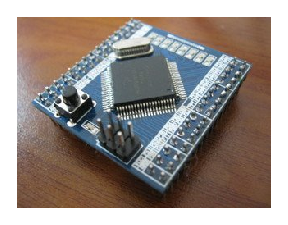
\includegraphics{chap3/coreminsys.eps}
  \bicaption{最小系统实物图}{最小系统实物图}{Fig}{the Minimal Core System}
\end{figure}
\begin{figure}[!htp]\label{fig.CoreSch}
  \centering
  \bicaption{最小系统电路图}{最小系统电路图}{Fig}{Schematic of the Minimal Core System}
  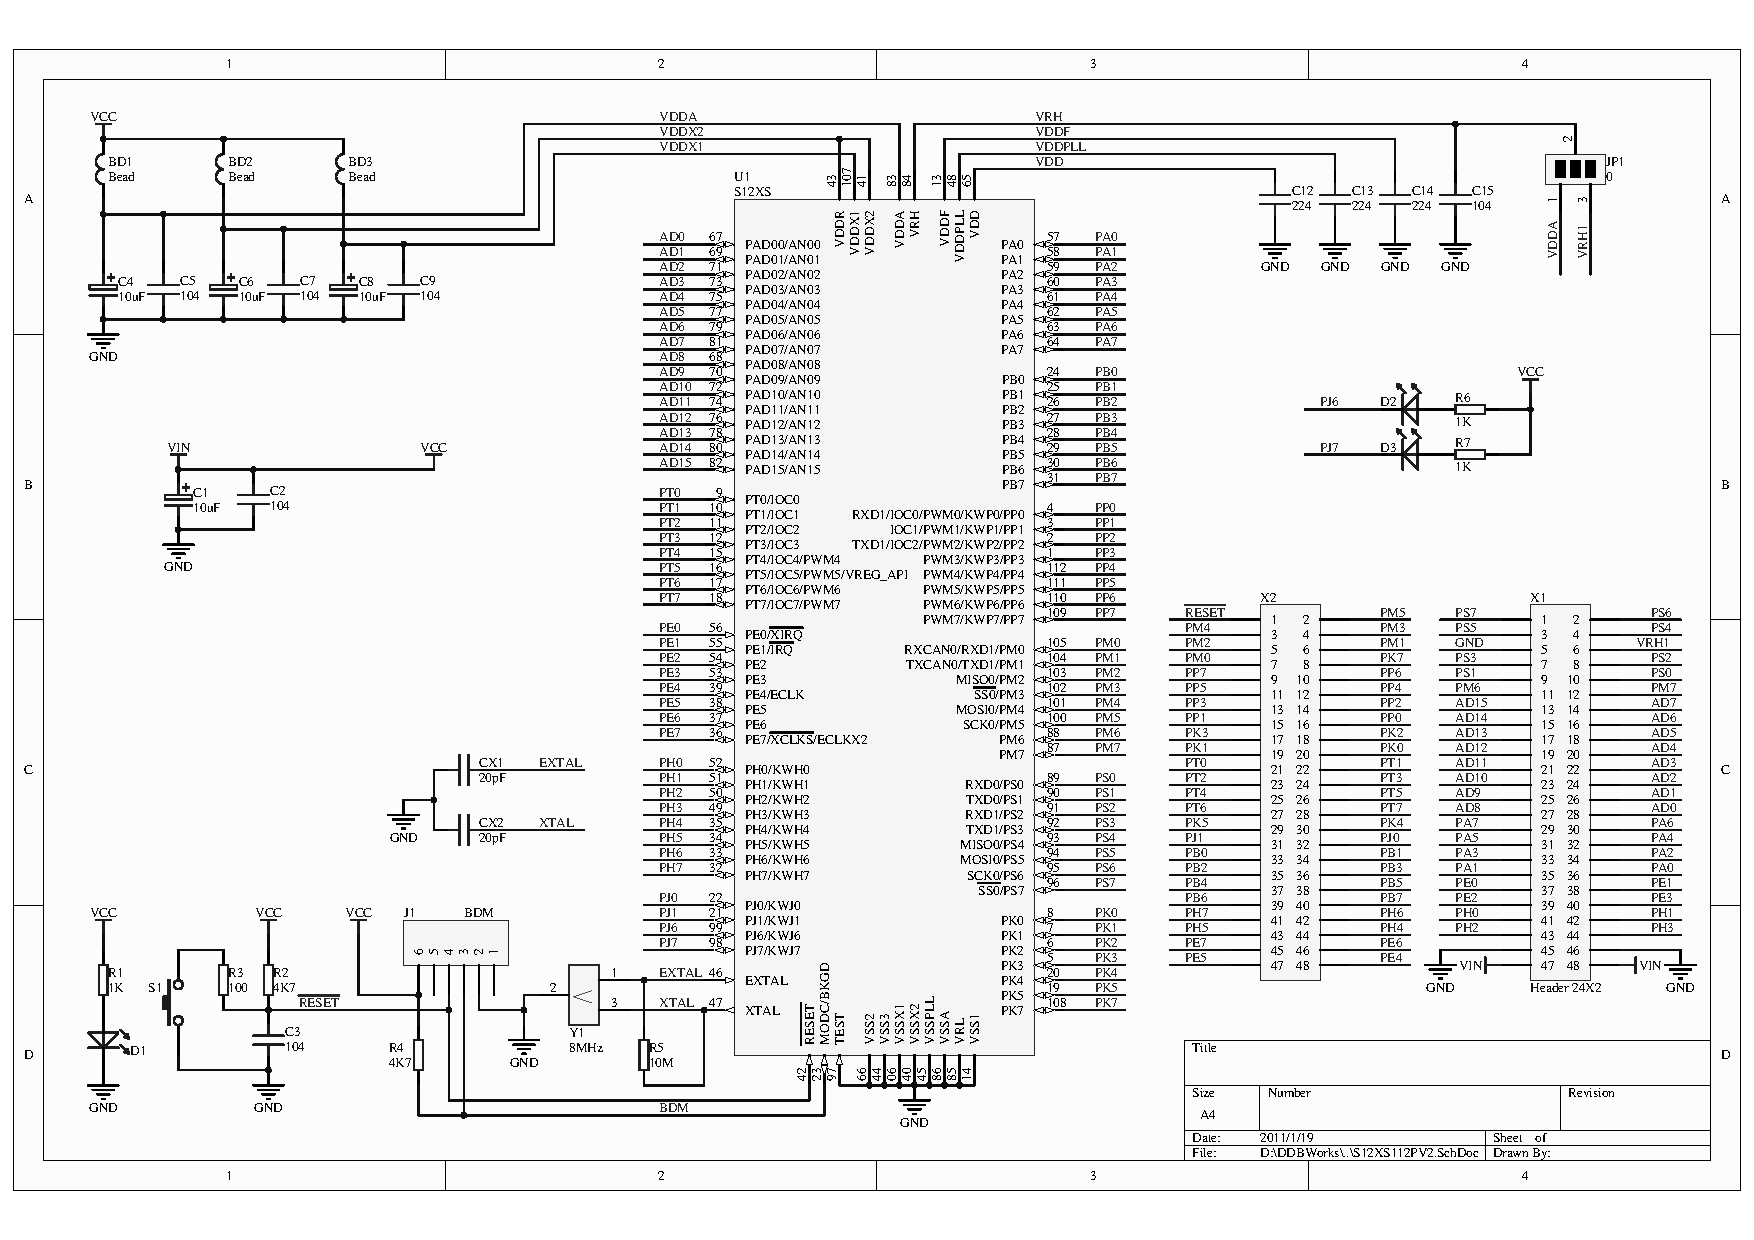
\includegraphics[angle=-90,width=1.3\textwidth]{chap3/Core112V2.pdf}
\end{figure}

这块最小系统板上有一个16MHz的晶振连接至芯片。芯片正常工作时的频率是由锁相环(PLL)超频到40MHz的。这块最小系统还有一个复位键,引入芯片RESET引脚,将检测电路的下降沿进行复位。同时最小系统上海提供一个BWM程序上传和下载及在线调试模块。片上提供128k片上RAM,可以用来储存芯片执行用程序。还有一个独立的电源管理模块,以提供稳定的5v电压给单片机工作。之所以称为最小系统,就是因为以上是这块芯片的全部功能元件。如原理图所示,这块最小系统的其他功能就是简单的将单片机所有引脚引出。 

\subsection{功能接口板}
功能接口板是通用模块控制电路的核心部分。它具有承上启下的作用,得到最小系统引出的单片机全部空余引脚,并对其功能进行设计。其电路图如图\ref{fig.BaseSch} 所示。 其共分为电源管理,CAN总线,单片机接口,电压测试单元,串口通讯,数码管显示单元,LED及案件阵列和引出接口几部分。 
\begin{figure}[!htp]\label{fig.BaseSch}
  \centering
  \bicaption{功能接口板电路图}{功能接口板电路图}{Fig}{Schematic of Base Board}
  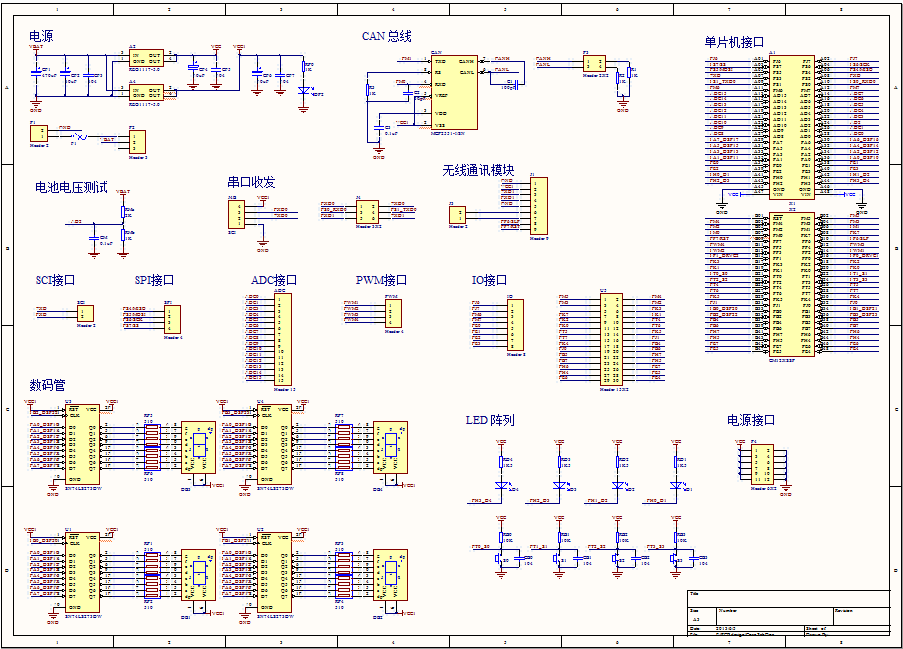
\includegraphics[angle=-90,width=0.8\textwidth]{chap3/CoreBoardSchematic.PNG}
\end{figure}


其中电源管理部分的电路如图\ref{fig.BaseScrMg}。使用两片1117输出两个5v电压,为了使电流相差较大模块之间不会相互干扰。其中一个给单片机及通讯模块供压,电流小,对电流稳定性要求高;而另一路主要给外设电路供压。 
\begin{figure}[!htp]\label{fig.BaseScrMg}
  \centering
  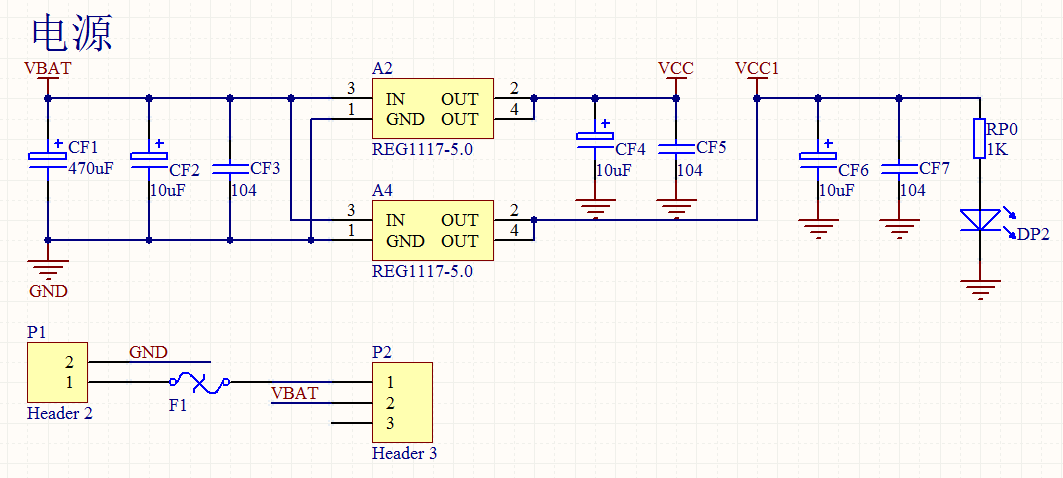
\includegraphics[width=0.8\textwidth]{chap3/CoreBoardPowerMg.PNG}
  \bicaption{电源管理电路原理图}{电源管理电路原理图}{Fig}{Schematic of Power Source Management Unit}
\end{figure}


CAN总线电路图如图所示\ref{fig.BaseCAN} 。用一块Microchip公司生产的MCP2511作为单片机内置CAN模块的Transceiver,将CAN端口数据打包编码后传输到总线中去。前面已经介绍过了这款机器人将打破传统的接触式传输连线,而是使用光学方法进行数据传输,其中这里CAN中线的输出口,就是要连接到光学传输接口板上。
\begin{figure}[!htp]\label{fig.BaseCAN}
  \centering
  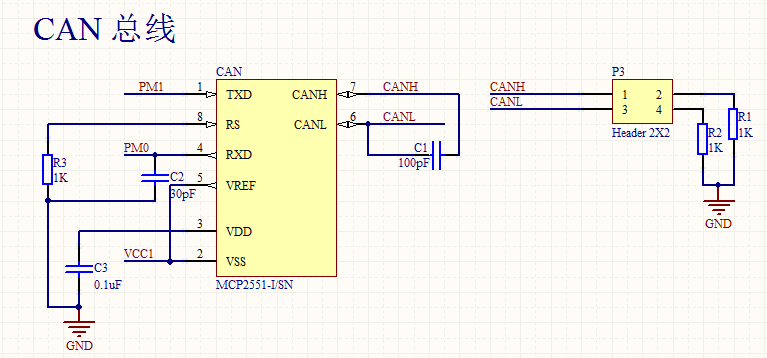
\includegraphics[width=0.8\textwidth]{chap3/CoreBoardCANBus.PNG}
  \bicaption{CAN电路原理图}{CAN电路原理图}{Fig}{Schematic of CAN Bus Unit}
\end{figure}


CAN总线2.0协议\upcite{bosch1991can}是由博世公司提出被提供支持的。因为其两线制的机制,和可以同时连接非常多个模块,并能组织各个节点模块共同工作的特点二大量应用在汽车领域。其传输速度快,稳定性强的特点也为其能轻松移植到机器人系统中来提供了可行性。相对较少的接线同时也意味着极大的容错率,这就是本设计选择CAN总线最为模块间传输工具的原因。这一设计的灵感来源于Ying Zhang等人\upcite{zhang2002massively}的研究。

功能接口板的PCB设计图如图\ref{fig.CorePCB} 所示。其虚拟实物图如图\ref{fig.CoreReal} 所示,3D立体仿真图如图\ref{fig.Core3D} 所示。 
\begin{figure}\label{fig.CorePCB}
  \centering
  \subfigure[PCB正面]{
    \label{fig:corepcb:a} %% label for first subfigure
    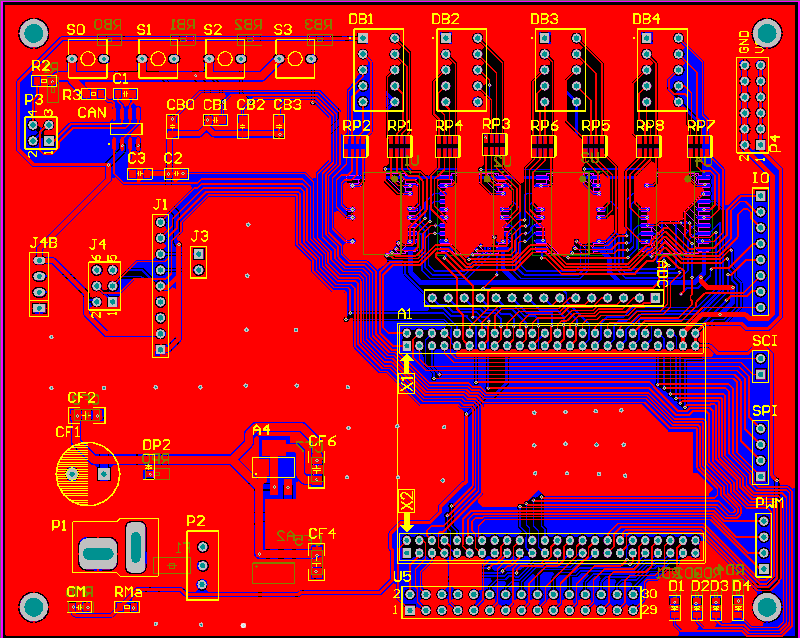
\includegraphics[width=0.35\textwidth]{chap3/CoreBoardTop.PNG}}
  \hspace{1in}
  \subfigure[PCB背面]{
    \label{fig:corepcb:b} %% label for second subfigure
    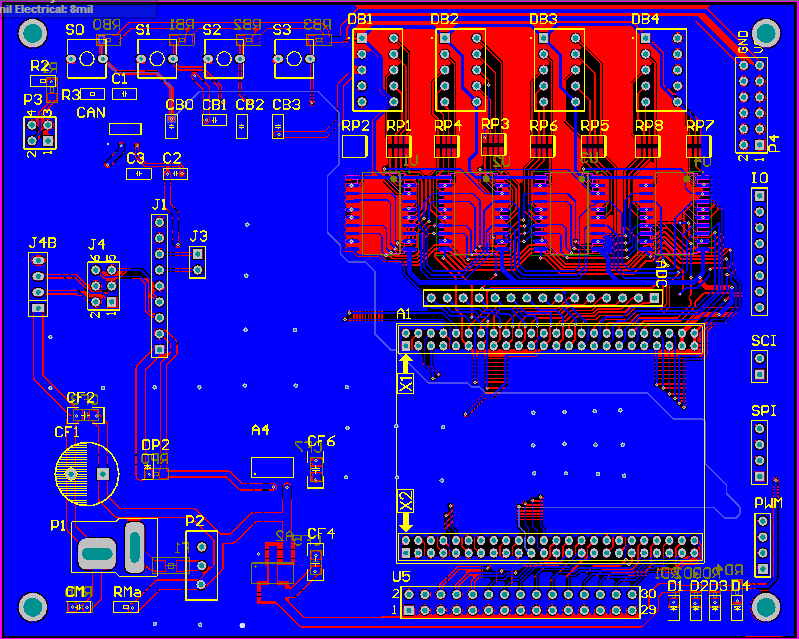
\includegraphics[width=0.35\textwidth]{chap3/CoreBoardBottom.PNG}}
  \bicaption{功能接口板的设计PCB样图}{功能接口板的设计PCB样图}{Fig}{The PCB View of Main Base Board}
\end{figure}
\begin{figure}\label{fig.CoreReal}
  \centering
  \subfigure[PCB正面]{
    \label{fig:corereal:a} %% label for first subfigure
    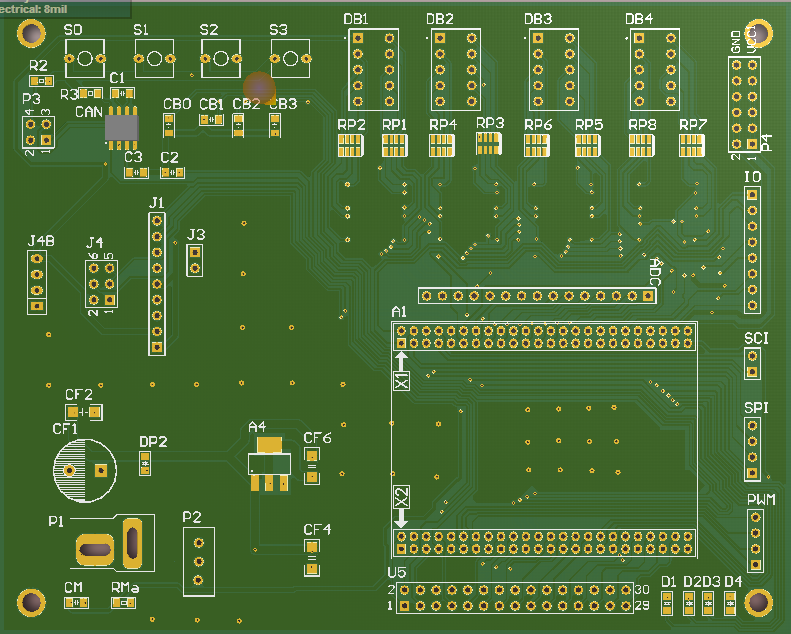
\includegraphics[width=0.35\textwidth]{chap3/CoreBoardManTop.PNG}}
  \hspace{1in}
  \subfigure[PCB背面]{
    \label{fig:corereal:b} %% label for second subfigure
    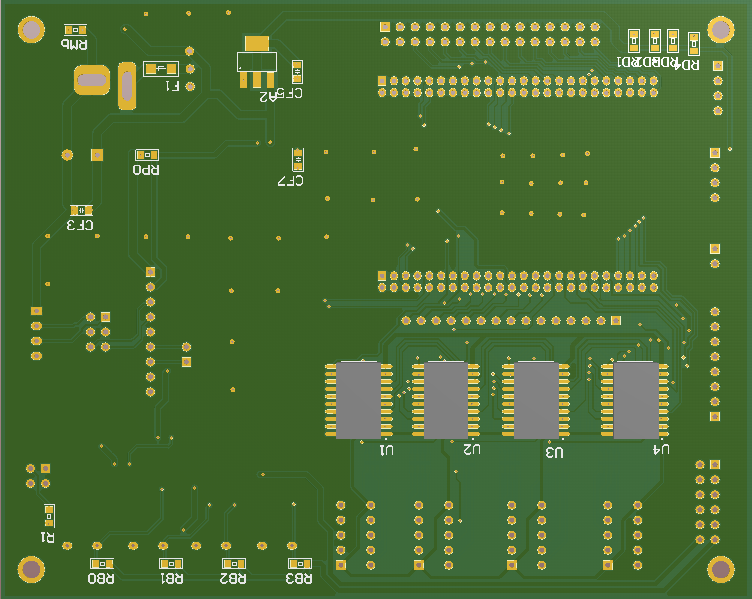
\includegraphics[width=0.35\textwidth]{chap3/CoreBoardManBottom.PNG}}
  \bicaption{功能接口板的虚拟实物图}{功能接口板的虚拟实物图}{Fig}{The Virtual View of Main Base Board}
\end{figure}
\begin{figure}[!htp]\label{fig.Core3D}
  \centering
  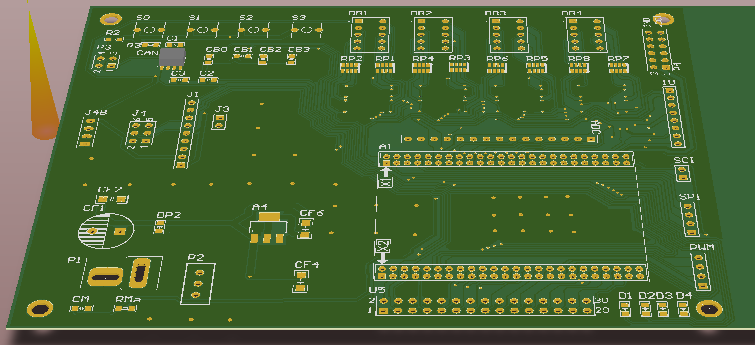
\includegraphics[width=0.8\textwidth]{chap3/CoreBoard3D.PNG}
  \bicaption{功能接口板的虚拟实物图3D}{功能接口板的虚拟实物图3D}{Fig}{The 3D Virtual View of Main Base Board}
\end{figure}
\section{功能型外设及接口设计}
功能性外设主要提供某个模块所需要的独特功能。这些模块可能包括机器人应用中的方方面面。如无线通讯模块:用来是摸个机器人模块与外部设备,如远程计算通讯,从而实现信息的沟通或是机器人于远程系统的交互;舵机驱动模块:可以用来驱动具有多舵机结构的机械臂或其他的多舵机应用模块;IMU和GPS模块:用来实现定位,机器人姿态探测等功能;电机驱动模块,用来驱动电机,可以用在轮式底盘或是履带式底盘的驱动;编码器模块:可以用来对固定于某一电机或伺服电机舵机上的编码器进行驱动与计数;传感器模块:用来驱动传感器来对外部信息进行采集和处理;以及其他应用领域的模块等等。本设计因为只对移动平台进行了设计及研究,所以只具体设计了IMU模块,电机驱动模块,编码器模块,传感器模块和光电CAN传输模块。对于每一个模块的详细设计如下。

\subsection{IMU模块}
IMU是Inertial measurement unit(惯性测量单元)的缩写。本方案所设计的IMU包括传统的加速度计和陀螺仪,同时参考了Minor等人\upcite{minor2001utilization}的设计,在模块中引入了磁倾角传感器(电子罗盘)。在这一模块的设计中,使用了一片SCA100T两轴角速度传感器,用来采集平行于地面的平面内的加速度;一个ZCC212N电子罗盘封装单元,这一单元将测得的与地磁场倾角数据通过SCI协议传输回单片机进行处理;以及一个LYPR540三轴陀螺仪,用以测量角加速度。电路设计原理图如图\ref{fig.IMUSch} 所示,PCB设计样图如图\ref{fig.IMUPCB} 所示,虚拟实物图如图\ref{fig.IMUReal} 所示。 
\begin{figure}[!htp]\label{fig.IMUSch}
  \centering
  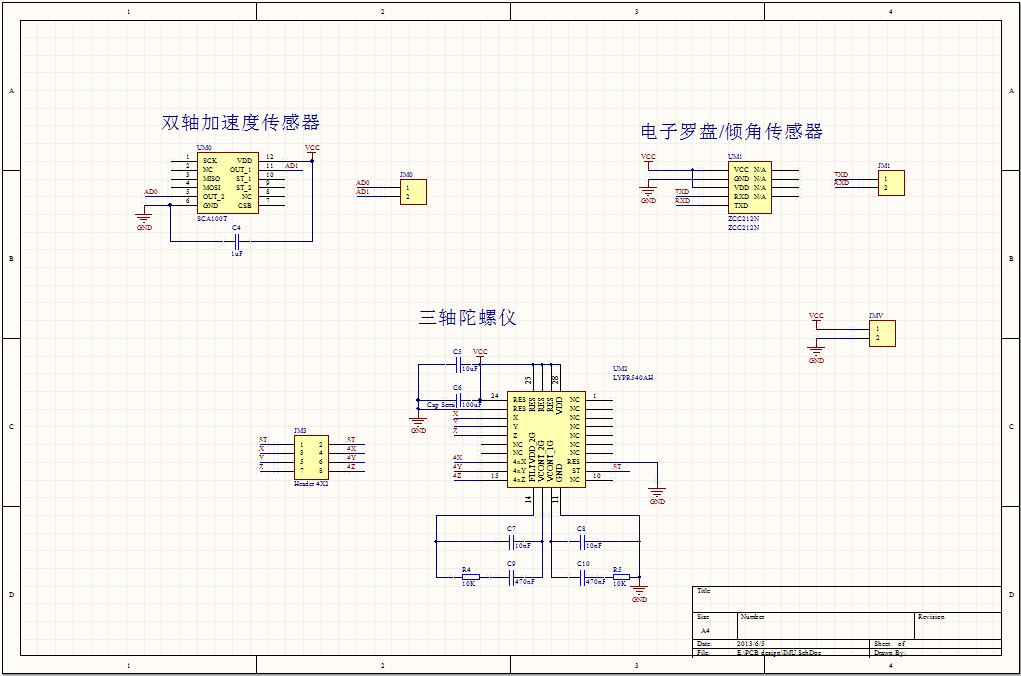
\includegraphics[angle=-90,width=0.8\textwidth]{chap3/IMU.PNG}
  \bicaption{IMU电路原理图}{IMU电路原理图}{Fig}{Schematic of IMU Unit}
\end{figure}
\begin{figure}\label{fig.IMUPCB}
  \centering
  \subfigure[PCB正面]{
    \label{fig:corepcb:a} %% label for first subfigure
    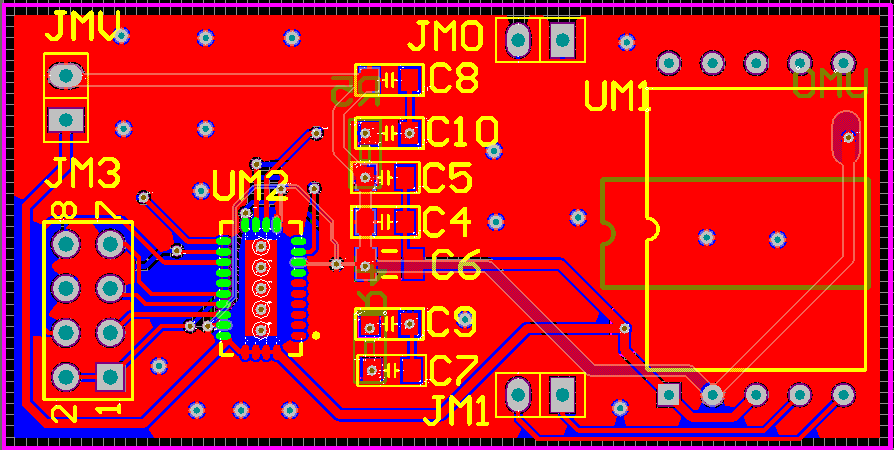
\includegraphics[width=0.35\textwidth]{chap3/IMUfront.PNG}}
  \hspace{1in}
  \subfigure[PCB背面]{
    \label{fig:corepcb:b} %% label for second subfigure
    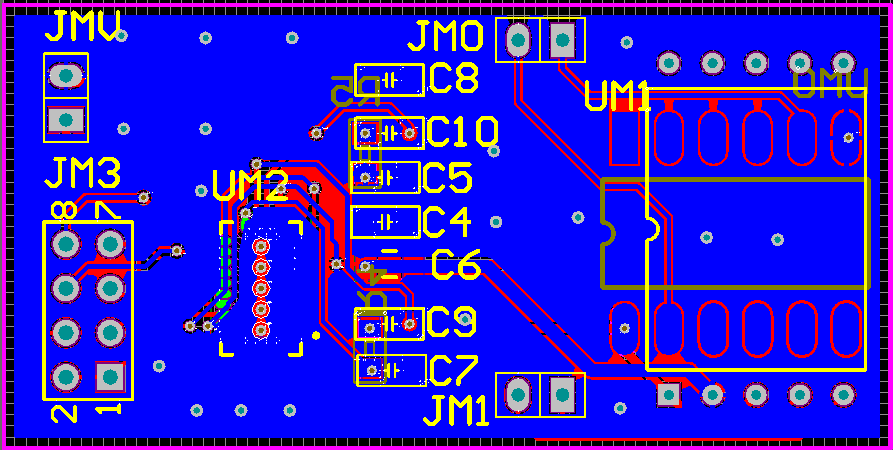
\includegraphics[width=0.35\textwidth]{chap3/IMUback.PNG}}
  \bicaption{IMU的设计PCB样图}{IMU的设计PCB样图}{Fig}{The PCB View of IMU}
\end{figure}
\begin{figure}\label{fig.IMUReal}
  \centering
  \subfigure[PCB正面]{
    \label{fig:corereal:a} %% label for first subfigure
    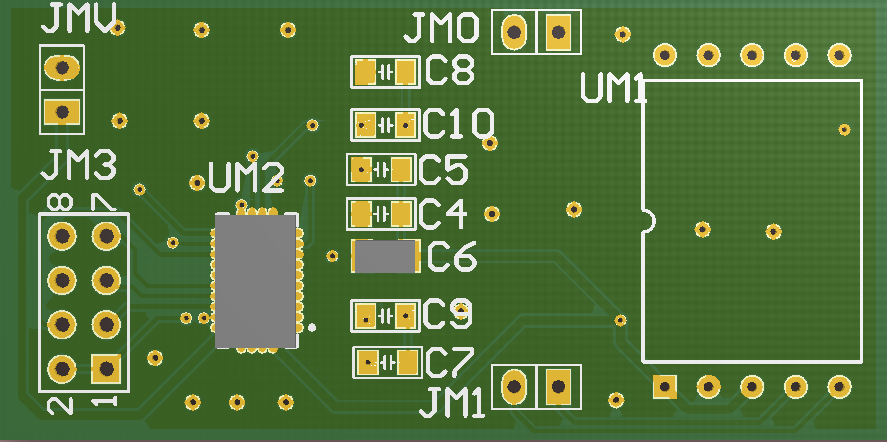
\includegraphics[width=0.35\textwidth]{chap3/IMUfrontVr.PNG}}
  \hspace{1in}
  \subfigure[PCB背面]{
    \label{fig:corereal:b} %% label for second subfigure
    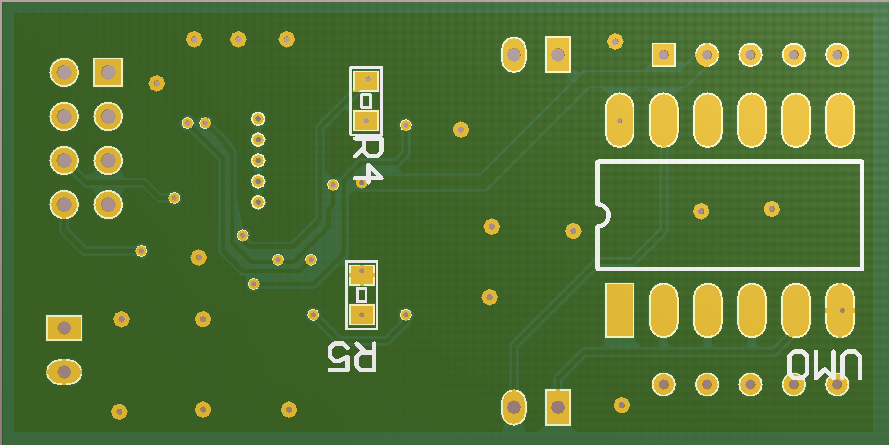
\includegraphics[width=0.35\textwidth]{chap3/IMUbackVr.PNG}}
  \bicaption{IMU的虚拟实物图}{IMU的虚拟实物图}{Fig}{The Virtual View of IMU}
\end{figure}

\subsection{驱动模块}
电机驱动模块,采用传统的H桥式电路。其电路原理简图如图\ref{fig.DrvPrinciple} 所示。 
\begin{figure}[!htp]\label{fig.DrvPrinciple}
  \centering
	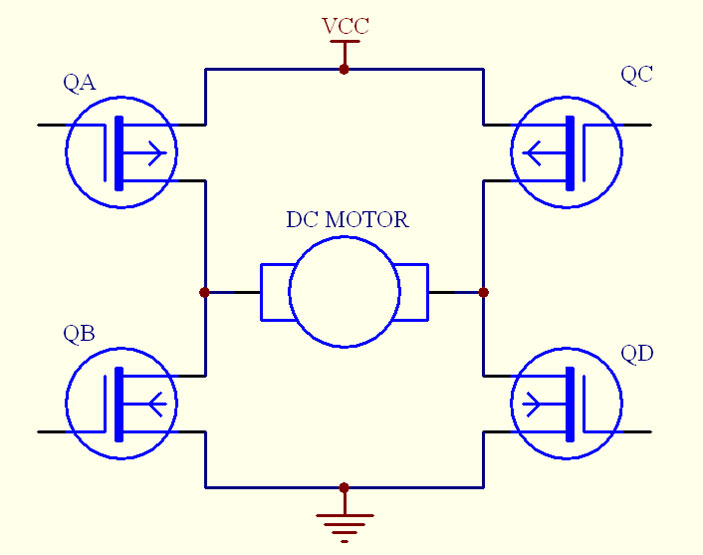
\includegraphics[width=0.3\textwidth]{chap3/H_Bridge.jpg}
	\bicaption{H桥电路原理简图}{H桥电路原理简图}{Fig}{H Bridge}
\end{figure}


其工作原理为,对角线上的MOSEFET或是BJT同时断开和闭合,相邻的两个MOSFET和BJT不同时断开和闭合。从而达到是电流可以以不同方向经过电机,而使电机可以正转或反转。现在有多种集成的桥式电路芯片可供选择,而不必用MOSFET自行搭建H桥式电路。这种集成芯片有多种好处,比如稳定性高,紧凑所占空间小,简化电路设计等。所以本方案的驱动电路是直接基于BTS7960这款H桥式芯片设计的。同时电机需要使用PWM脉冲调制器产生方波来进行控速,通过改变方波的占空比来改变作用在电机上的等效电压来实现调速。其原理图如图\ref{fig.Drv} 所示,PCB设计样图如图\ref{fig.DrvPCB} 所示。
\begin{figure}[!htp]\label{fig.Drv}
  \centering
  \bicaption{驱动电路电路图}{驱动电路电路图}{Fig}{Schematic of Driver Board}
  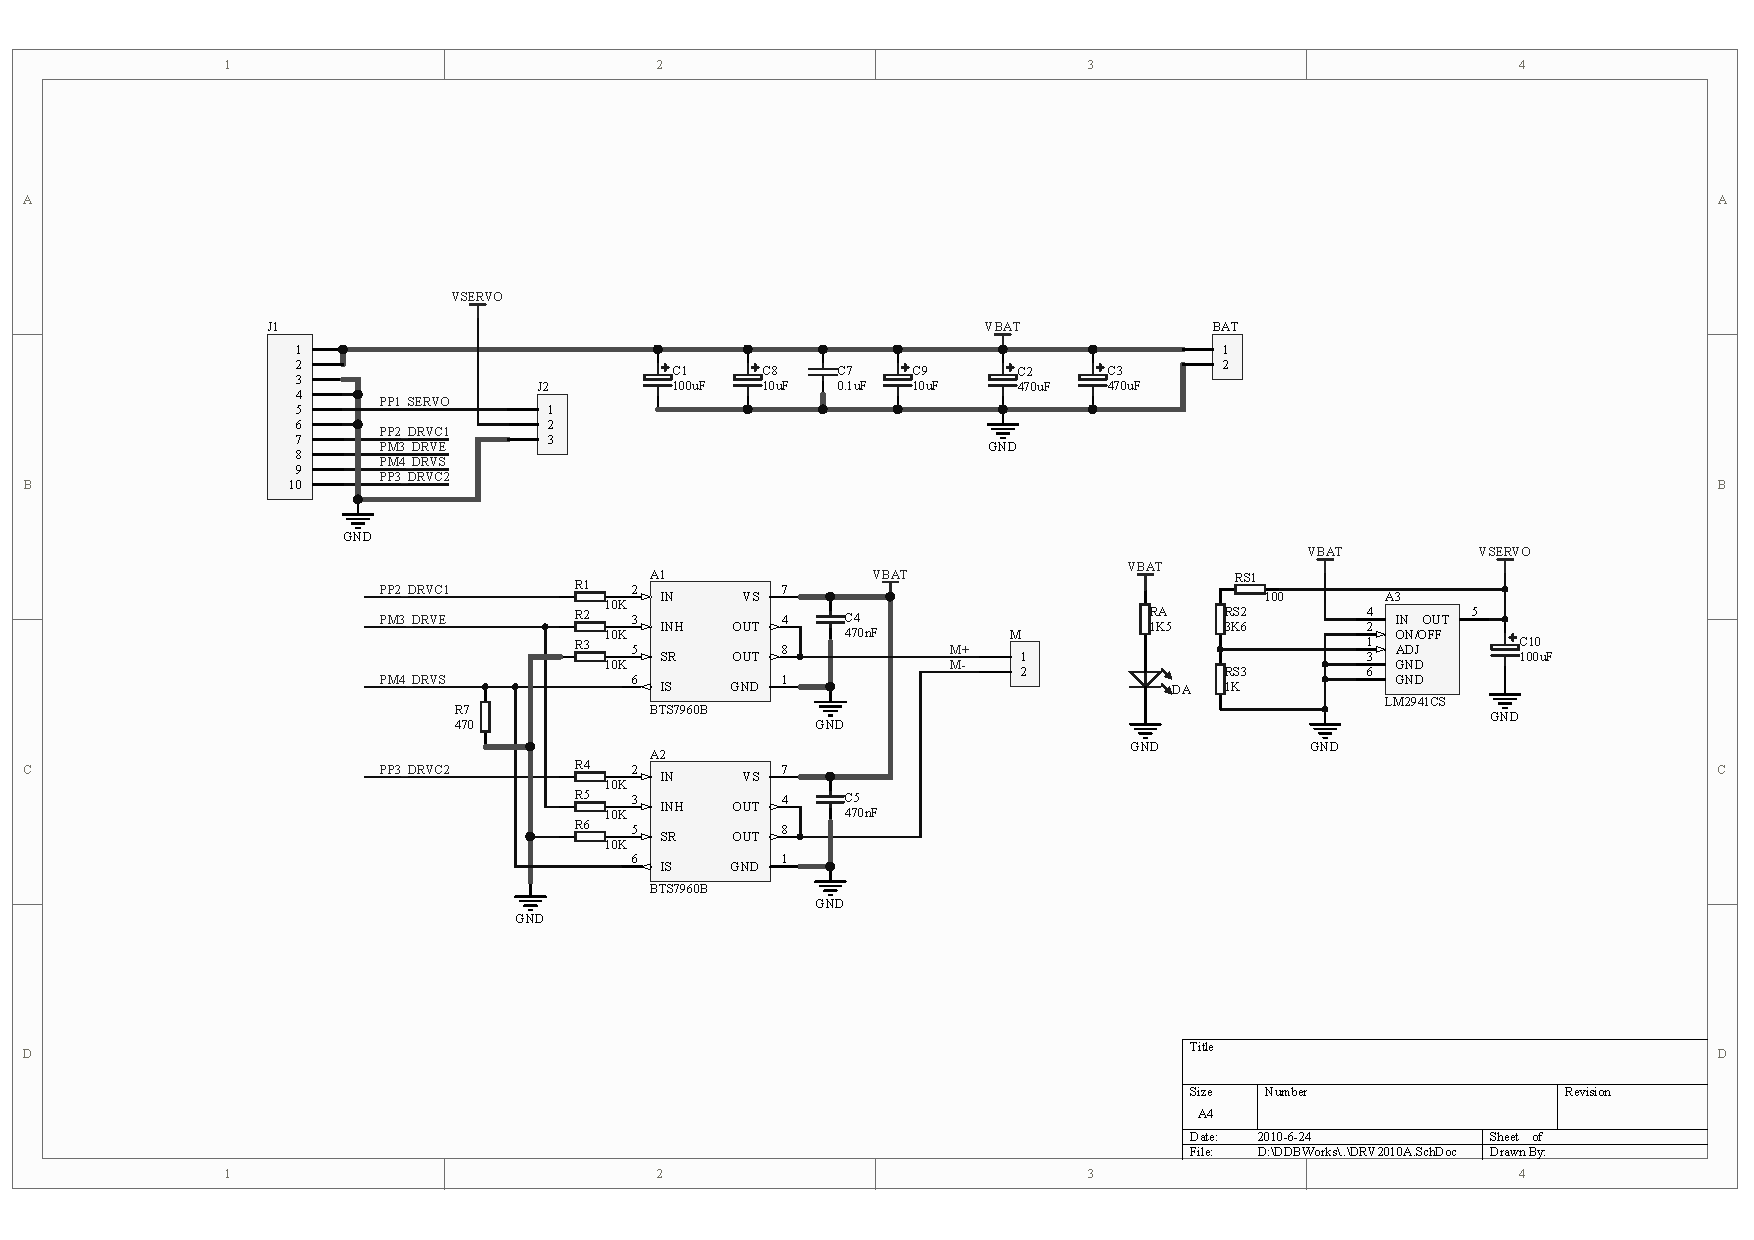
\includegraphics[angle=-90,width=0.8\textwidth]{chap3/DRV2010A.pdf}
\end{figure}
\begin{figure}\label{fig.DrvPCB}
  \centering
  \subfigure[PCB正面]{
    \label{fig:corepcb:a} %% label for first subfigure
    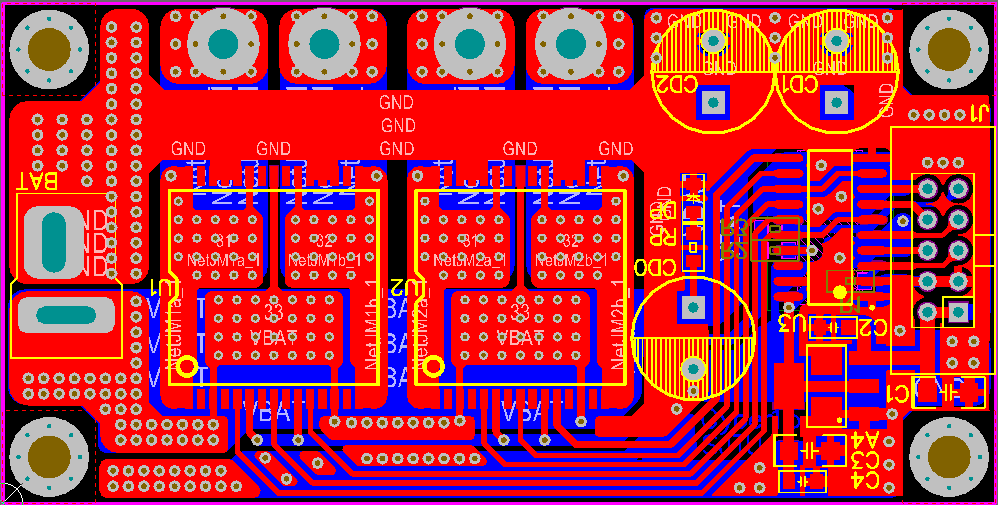
\includegraphics[width=0.35\textwidth]{chap3/DrvPCBTop.PNG}}
  \hspace{1in}
  \subfigure[PCB背面]{
    \label{fig:corepcb:b} %% label for second subfigure
    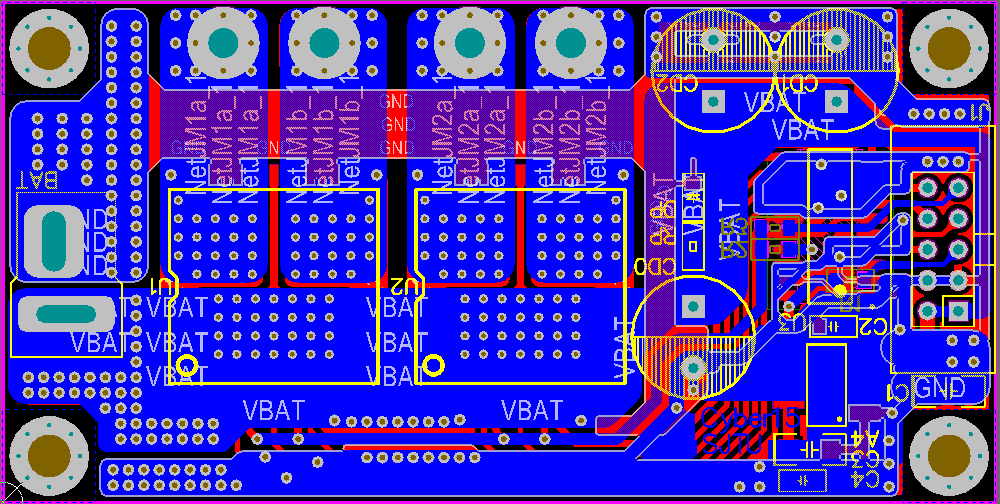
\includegraphics[width=0.35\textwidth]{chap3/DrvPCBBack.PNG}}
  \bicaption{驱动电路的设计PCB样图}{驱动电路的设计PCB样图}{Fig}{The PCB View of Driver Board}
\end{figure}

\subsection{编码器模块}
编码器模块实际上是比较简单的模块,其主要功能是为编码器提供片外计数器,并把结果反馈给主控板。在本设计中,选用的是CD4520芯片。这是一个最高计数值较小的高速用计数器。每个芯片的接线方法的电路原理图如图\upcite{ConSch}。\\
\begin{figure}[!htp]\label{fig.ConSch}
  \centering
  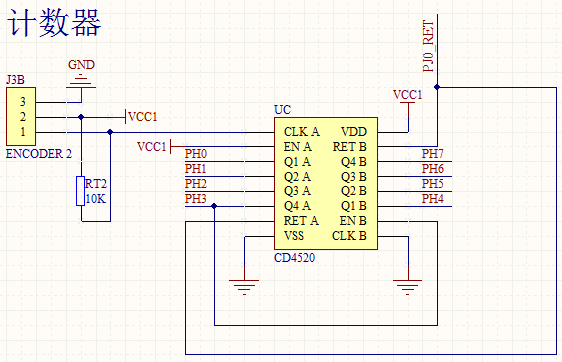
\includegraphics[width=0.8\textwidth]{chap3/counter.PNG}
  \bicaption{编码器用外部计数器接线图}{编码器用外部计数器接线图}{Fig}{Schematic of counters for encoder}
\end{figure}
\subsection{传感器模块}
传感器模块需要因传感器种类的不同而不同。在这里只对本设计需要用的超声波传感器的驱动电路进行讨论。因为传感器众多,为了节省片上资源,需要新的方法去驱动这么多传感器。其中一种方案就如笔者的设计,轮流激活传感器网络中的各个个体,这样可以复用同一套数据读取口,只需要不同的选通IO接口就可以了。这种方法充分的考虑到了片上资源不足的情况,极大的减少所要使用IO口的数量。传感器驱动网络的原理图如图\ref{fig.ultraSonic}所示。从图中可以看出PK7口是复用的,是有上升沿和下降沿检测中断的端口。如果使用译码器驱动选通的话,可以以供使用4个IO口驱动8个传感器。
\begin{figure}[!htp]\label{fig.ultraSonic}
  \centering
  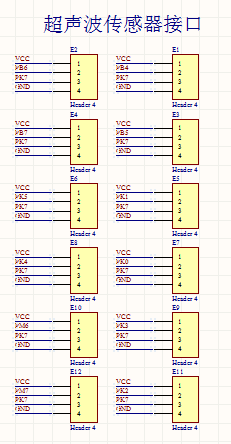
\includegraphics[width=0.4\textwidth]{chap3/ultraSonic.PNG}
  \bicaption{超声波传感器驱动板原理图}{超声波传感器驱动板原理图}{Fig}{Schematic of Ultrasonics Driver Unit}
\end{figure}


在本设计中选用的传感器是比较常见的HC-SR04模块。其有效检测距离是4cm到8m。超声波传感器不同于红外传感器,抗光线和环境干扰能力比较强,相对可靠。同时因为模块的常见性,又使其非常廉价。这款模块的实物图如图\ref{fig.ultraSonicReal} 所示。 \\
\begin{figure}[!htp]\label{fig.ultraSonicReal}
  \centering
  \subfigure[正面]{
    \label{fig:corepcb:a} %% label for first subfigure
    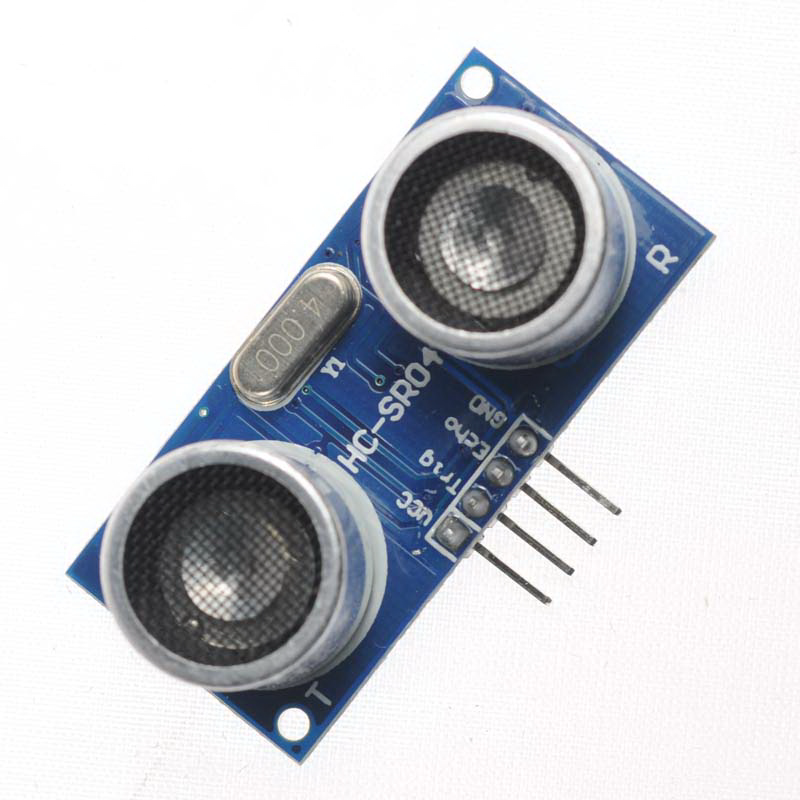
\includegraphics[width=0.35\textwidth]{chap3/HC_SR04.png}}
  \hspace{1in}
  \subfigure[背面]{
    \label{fig:corepcb:b} %% label for second subfigure
    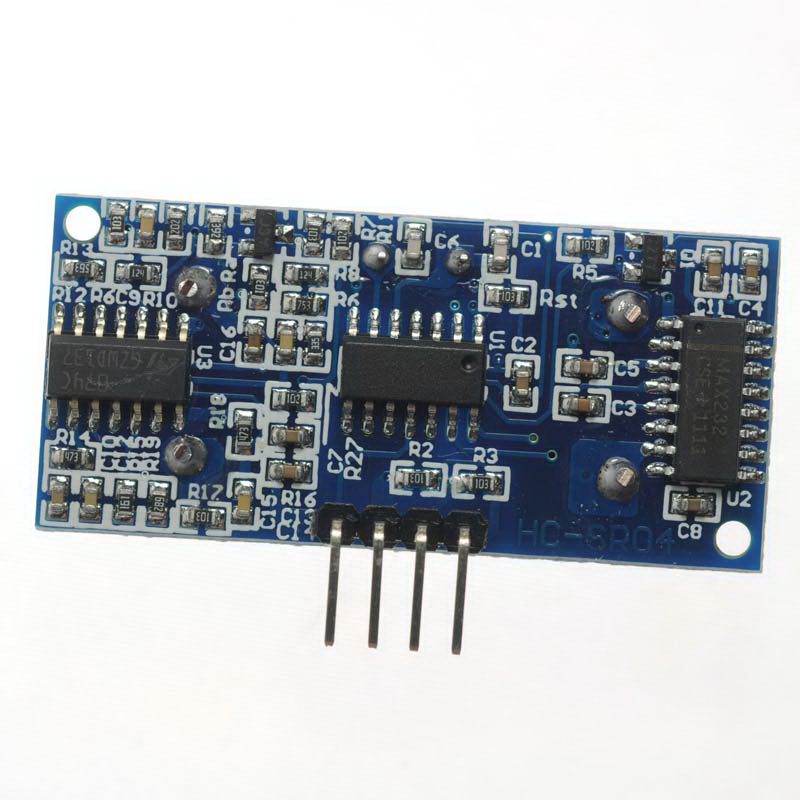
\includegraphics[width=0.35\textwidth]{chap3/HC_SR04back.png}}
  \bicaption{超声波传感器}{超声波传感器}{Fig}{Ultrasonics Sensor Unit}
\end{figure}
\subsection{模块间通讯接口}
\section{本章小结}

